%% LyX 2.3.6.1 created this file.  For more info, see http://www.lyx.org/.
%% Do not edit unless you really know what you are doing.
\documentclass[english]{article}
\usepackage[T1]{fontenc}
\usepackage[latin9]{inputenc}
\usepackage{geometry}
\geometry{verbose,tmargin=2.5cm,bmargin=2.5cm,lmargin=2.5cm,rmargin=2.5cm}
\usepackage{graphicx}
\PassOptionsToPackage{normalem}{ulem}
\usepackage{ulem}

\makeatletter

%%%%%%%%%%%%%%%%%%%%%%%%%%%%%% LyX specific LaTeX commands.
%% Because html converters don't know tabularnewline
\providecommand{\tabularnewline}{\\}

\makeatother

\usepackage{babel}
\begin{document}
{[}SPLIT\_HERE{]}
\begin{enumerate}
\item \textbf{{[}RVHS/PRELIM/9597/2019/P1/Q1{]} }

\textbf{CID3 Team Grouping} 

In this question, you will help the CID3 students in forming CID3
groups for their projects. 

In \textquotedblleft \texttt{student\_cid.txt}\textquotedblright{} 

There are three fields on each line which indicates \texttt{name},
\texttt{role} and \texttt{gender} of 50 cid3 students. The fields
are separated by \textquoteleft ;\textquoteright{} 

\noindent %
\noindent\begin{minipage}[t]{1\columnwidth}%
\texttt{Rufus Schuck;Coder;F }

\texttt{Ione Wolfe;Dealer;F }

\texttt{Hillary Curl;Coder;M }

\texttt{\dots{} }%
\end{minipage}

\subsection*{Task 1.1 }

Implement the function \texttt{read\_data(filename)} which takes \texttt{filename}
as a string and returns a 2-dimension list that follows the format
as shown in the example below.

\noindent %
\noindent\begin{minipage}[t]{1\columnwidth}%
\texttt{>\textcompwordmark >\textcompwordmark > read\_data(\textquotedbl student\_cid.txt\textquotedbl ) }

\texttt{{[}{[}'Rufus Schuck', 'Coder', 'F'{]}, {[}'Ione Wolfe', 'Dealer',
'F'{]}, {[}'Hillary Curl', 'Coder', 'M'{]},\dots {]} }%
\end{minipage}

\subsection*{Evidence 1 }

Program code of function \texttt{read\_data}. \hfill{}{[}2{]}

\subsection*{Task 1.2}

Implement the function \texttt{gender\_count(cid\_student\_lst, is\_female)}
which takes a list \texttt{cid\_student\_lst} and a boolean \texttt{is\_female}
as inputs and returns the number of female students in \texttt{cid\_student\_lst}
if \texttt{is\_female} is \texttt{True}, otherwise return the number
of male students. \texttt{cid\_student\_lst} is the list obtained
in \textbf{Task 1.1}. 

\subsection*{Evidence 2 }

Program code of function \texttt{gender\_count}.\hfill{} {[}2{]}

\subsection*{Evidence 3 }

Screenshot of the output of the following: 

\noindent %
\noindent\begin{minipage}[t]{1\columnwidth}%
\texttt{cid\_student\_lst = read\_data(\textquotedbl student\_cid.txt\textquotedbl ) }

\texttt{print(gender\_count(cid\_student\_lst, True)) }

\texttt{print(gender\_count(cid\_student\_lst, False))}\hfill{}\texttt{
}{[}1{]}%
\end{minipage}

\subsection*{Task 1.3 }

Implement the procedure \texttt{role\_statistics(cid\_student\_lst)}
which takes a list \texttt{cid\_student\_lst} as input and output
the number of students for each role in the following format. (There
are more than 5 types of roles.) 

For example: 

\noindent %
\noindent\begin{minipage}[t]{1\columnwidth}%
\texttt{>\textcompwordmark >\textcompwordmark > cid\_student\_lst
= read\_data(\textquotedbl student\_cid.txt\textquotedbl ) }

\texttt{>\textcompwordmark >\textcompwordmark > role\_statistics(cid\_student\_lst) }

\texttt{Role ~~~~~~~Number }

\texttt{Coder ~~~~~~11 }

\texttt{Dealer ~~~~~13 }

\texttt{Designer ~~~14 }

\texttt{Empathizer ~14 }

\texttt{Maker ~~~~~~12 }%
\end{minipage}

Take note that the roles and numbers shown above is just an example.

\subsection*{Evidence 4 }

Program code of procedure \texttt{role\_statistics}.\hfill{} {[}3{]}

\subsection*{Evidence 5}

Screenshot of the output of the following: 

\noindent %
\noindent\begin{minipage}[t]{1\columnwidth}%
\texttt{cid\_student\_lst = read\_data(\textquotedbl student\_cid.txt\textquotedbl ) }

\texttt{role\_statistics(cid\_student\_lst)}\hfill{} {[}1{]}%
\end{minipage}

\subsection*{Task 1.4 }

Implement the function \texttt{form\_random\_group(cid\_student\_lst)}
which takes a list \texttt{cid\_student\_lst} as input and returns
a list consists of 5 student names. This list of students forms a
group and must consist of one coder, one maker, one dealer, one empathizer
and one designer. The student picked for each role must be random.
If there is not sufficient roles or students to form a group, return
an empty list. 

For example: 

\noindent %
\noindent\begin{minipage}[t]{1\columnwidth}%
\texttt{>\textcompwordmark >\textcompwordmark > cid\_student\_lst
= read\_data(\textquotedbl student\_cid.txt\textquotedbl ) }

\texttt{>\textcompwordmark >\textcompwordmark > form\_random\_group(cid\_student\_lst) }

\texttt{{[}'Fredricka Gormley', 'Jalisa Stoudemire', 'Laverna Halpern',
'Chadwick Griffin', 'Abdul Boland'{]} }%
\end{minipage}

Note: 

\noindent %
\noindent\begin{minipage}[t]{1\columnwidth}%
\texttt{Fredricka Gormley is a coder }

\texttt{Jalisa Stoudemire is a dealer}

\texttt{Laverna Halpern is a designer }

\texttt{Chadwick Griffin is an empathizer }

\texttt{Abdul Boland is a maker}%
\end{minipage}

\subsection*{Evidence 6 }

Program code of procedure \texttt{form\_random\_group}.\hfill{} {[}5{]}

\subsection*{Evidence 7 }

Screenshot of the output of the following: 

\noindent %
\noindent\begin{minipage}[t]{1\columnwidth}%
\texttt{cid\_student\_lst = read\_data(\textquotedbl student\_cid.txt\textquotedbl ) }

\texttt{for i in range(3): }

\texttt{\qquad{}print(form\_random\_group(cid\_student\_lst))} \hfill{}{[}1{]}%
\end{minipage}

\subsection*{Task 1.5 }

Implement the function \texttt{remove\_students} which takes \texttt{cid\_student\_lst}
and \texttt{one\_cid\_group} as inputs where \texttt{cid\_studnet\_lst}
is the list obtained from \textbf{task 1.1} and \texttt{one\_cid\_group}
is the list of 5 student names obtained from task 1.4. The function
removes 5 records in \texttt{cid\_student\_lst} specified by the student
names in \texttt{one\_cid\_group} and returns the removed records
in a list. For example: 

\noindent %
\noindent\begin{minipage}[t]{1\columnwidth}%
\texttt{>\textcompwordmark >\textcompwordmark > cid\_student\_lst
= read\_data(\textquotedbl student\_cid.txt\textquotedbl )}

\texttt{>\textcompwordmark >\textcompwordmark > one\_cid\_group
= form\_random\_group(cid\_student\_lst) }

\texttt{>\textcompwordmark >\textcompwordmark > one\_cid\_group
{[}'Rufus Schuck', 'Kathlene Collar', 'Luanne Lett', 'Phyliss Rolen',
'Tobias Kimmer'{]} }

\texttt{>\textcompwordmark >\textcompwordmark > remove\_students(cid\_student\_lst,
one\_cid\_group) {[}{[}'Rufus Schuck', 'Coder', 'F'{]}, {[}'Kathlene
Collar', 'Empathizer', 'M'{]}, {[}'Luanne Lett', 'Dealer', 'F'{]},
{[}'Phyliss Rolen', 'Maker', 'M'{]}, {[}'Tobias Kimmer', 'Designer',
'F'{]}}

\texttt{>\textcompwordmark >\textcompwordmark > len(cid\_student\_lst) }

\texttt{45 }%
\end{minipage}

After \texttt{remove\_students(cid\_student\_lst, one\_cid\_group)}
is executed \texttt{cid\_student\_lst} should not contain any records
with students name \texttt{Fredricka Gormley}, \texttt{Jalisa Stoudemire},
\texttt{Laverna Halpern}, \texttt{Chadwick Griffin} and \texttt{Abdul
Boland}. Since the 5 names are removed. \texttt{cid\_student\_lst}
should now have 45 records. 

\subsection*{Evidence 8 }

Program code of function \texttt{remove\_students}. \hfill{}{[}4{]}

\subsection*{Evidence 9 }

Screenshot of the output of the following code. 

\noindent %
\noindent\begin{minipage}[t]{1\columnwidth}%
\texttt{def test\_15(): }

\texttt{\qquad{}print(\textquotedbl -{}-{}-{}-{}-{}-Task 1.5-{}-{}-{}-{}-{}-\textquotedbl ) }

\texttt{\qquad{}cid\_student\_lst = read\_data(\textquotedbl student\_cid.txt\textquotedbl ) }

\texttt{\qquad{}one\_cid\_group = form\_random\_group(cid\_student\_lst) }

\texttt{\qquad{}removed\_records = remove\_students(cid\_student\_lst,
one\_cid\_group) }

\texttt{\qquad{}print(\textquotedbl removed records\textquotedbl ) }

\texttt{\qquad{}for removed\_record in removed\_records: }

\texttt{\qquad{}\qquad{}print(removed\_record) }

\texttt{\qquad{}print(\textquotedbl remaining records\textquotedbl ) }

\texttt{\qquad{}for cid\_student in cid\_student\_lst: }

\texttt{\qquad{}\qquad{}print(cid\_student) }

\texttt{test\_15()} \hfill{} {[}1{]}%
\end{minipage}

\subsection*{Task 1.6 }

Using your solutions in task 1.1, 1.4 and 1.5, write a procedure \texttt{form\_max\_cid\_group}
which takes a list \texttt{cid\_student\_lst} as input and write to
a file named \textquotedblleft \texttt{result.txt}\textquotedblright{}
the suggested maximum number of CID3 groups that can be formed from
\texttt{cid\_student\_lst}. The content in \textquotedbl\texttt{result.txt}\textquotedbl{}
should also include the group number and its group members. For example,
the content of \textquotedbl\texttt{result.txt}\textquotedbl{} can
be: 

\noindent %
\noindent\begin{minipage}[t]{1\columnwidth}%
\texttt{Group 0}

\texttt{Rufus Schuck Coder F}

\texttt{Lashawna Meals Dealer M}

\texttt{Phyliss Rolen Maker M }

\texttt{Laverna Halpern Designer F }

\texttt{Apryl Soileau Empathizer F }

\texttt{Group 1 }

\texttt{Claudette Bode Maker F }

\texttt{Angle Linck Coder F }

\texttt{Grazyna Kitzman Designer M }

\texttt{Virgilio Britt Dealer F }

\texttt{Dannette Raasch Empathizer F }

\texttt{Group 2 }

\texttt{Carolann Kintner Designer M }

\texttt{Ola Markell Empathizer F }

\texttt{Jaye Galle Maker F }

\texttt{Lanita Sciortino Coder M}

\texttt{Joella Wessner Dealer F }

\texttt{Group 3 }

\texttt{Hertha Dossantos Dealer F }

\texttt{Chadwick Griffin Empathizer M }

\texttt{Fredricka Gormley Coder F }

\texttt{Marcella Daigneault Designer F}

\texttt{Farah Quon Maker F}

\texttt{Group 4 }

\texttt{Hillary Curl Coder M }

\texttt{Elvia Dubrey Designer F}

\texttt{Terrence Shannon Empathizer M }

\texttt{Luanne Lett Dealer F }

\texttt{See Borne Maker F }

\texttt{Group 5 }

\texttt{Toney Mcnab Coder M }

\texttt{Jalisa Stoudemire Dealer M }

\texttt{Abdul Boland Maker M }

\texttt{Russell Gillison Designer F }

\texttt{Reiko Stack Empathizer F}%
\end{minipage}

\subsection*{Evidence 10 }

Program code of procedure \texttt{form\_max\_cid\_group}. \hfill{}{[}4{]}

\subsection*{Evidence 11 }

Screenshot of the content of \textquotedbl\texttt{result.txt}\textquotedbl .
\hfill{}{[}1{]}

{[}SPLIT\_HERE{]}
\item \textbf{{[}RVHS/PRELIM/9597/2019/P1/Q2{]} }

\textbf{EAN-13 }

EAN-13 (European Article Number) barcode a standard describing a barcode
symbology and numbering system used in global trade to identify a
specific retail product type, in a specific packaging configuration,
from a specific manufacturer. 

EAN check digits are calculated by summing each of the odd position
numbers multiplied by 3 and then by adding the sum of the even position
numbers. 

Numbers are examined going from right to left, so the first odd position
is the last digit in the code. The final digit of the result is subtracted
from 10 to calculate the check digit. 

For example, 

\noindent %
\noindent\begin{minipage}[t]{1\columnwidth}%
\texttt{EAN(first 12 digits) = }\texttt{\textbf{4}}\texttt{0}\texttt{\textbf{0}}\texttt{6}\texttt{\textbf{3}}\texttt{8}\texttt{\textbf{1}}\texttt{3}\texttt{\textbf{3}}\texttt{3}\texttt{\textbf{9}}\texttt{3 }

\texttt{Even digits ~~~~~~~~~= 4 + 0 + 3 + 1 + 3 + 9 ~~~~~~=
20 }

\texttt{Odd digits x 3 ~~~~~~= (0 + 6 + 8 + 3 + 3 + 3) x 3 =
69 }

\texttt{Total ~~~~~~~~~~~~~~~= 20 + 69 ~~~~~~~~~~~~~~~~~~~~=
89 }

\texttt{Check digit ~~~~~~~~~= 10 \textendash{} 9 ~~~~~~~~~~~~~~~~~~~~~=
1 }%
\end{minipage}

Therefore, the valid EAN number is \texttt{4006381333931}. 

\subsection*{Task 2.1 }

Implement the \textbf{\emph{iterative}} function \texttt{EAN} that
takes in a string \texttt{ean12} which is the first 12 characters
of a valid EAN number and returns the full valid EAN with the check
digit in string. 

For example:

\noindent %
\noindent\begin{minipage}[t]{1\columnwidth}%
\texttt{>\textcompwordmark >\textcompwordmark > EAN(\textquotedbl 400638133393\textquotedbl ) }

\texttt{\textquotedbl 4006381333931\textquotedbl{} }

\texttt{>\textcompwordmark >\textcompwordmark > EAN(\textquotedbl 590123412345\textquotedbl )}

\texttt{\textquotedbl 5901234123457\textquotedbl{} }%
\end{minipage}

\subsection*{Evidence 12 }

Program code for \texttt{EAN}. \hfill{} {[}3{]}

\subsection*{Evidence 13 }

Screenshot of the output of the following code. \hfill{} {[}1{]}

\noindent %
\noindent\begin{minipage}[t]{1\columnwidth}%
\texttt{print(EAN(\textquotedbl 400638133393\textquotedbl ))}

\texttt{print(EAN(\textquotedbl 590123412345\textquotedbl )) }

\texttt{print(EAN(\textquotedbl 950110153000\textquotedbl )) }

\texttt{print(EAN(\textquotedbl 007567816412\textquotedbl )) }

\texttt{print(EAN(\textquotedbl 123456789123\textquotedbl )) }

\texttt{print(EAN(\textquotedbl 563643712973\textquotedbl )) }%
\end{minipage}

\subsection*{Task 2.2}

Implement the function \texttt{EAN\_rec} which is the recursive version
of task 2.1. 

\subsection*{Evidence 14}

Program code for \texttt{EAN\_rec}. \hfill{}{[}3{]}

\subsection*{Task 2.3 }

Implement the function \texttt{generate\_n\_random\_EAN(n)} that takes
an integer \texttt{n} as input and return a list that contains n random
valid EAN numbers in string. 

For example: 

\noindent %
\noindent\begin{minipage}[t]{1\columnwidth}%
\texttt{>\textcompwordmark >\textcompwordmark > generate\_n\_random\_EAN(5)}

\texttt{{[}'9399783016850', '7126497037138', '7859230985143', '4663965860605',
'0075678464126'{]}}%
\end{minipage}

\subsection*{Evidence 15 }

Program code for \texttt{generate\_n\_random\_EAN}. \hfill{} {[}3{]}

\subsection*{Evidence 16 }

Screenshot of the output of the following code: \hfill{} {[}1{]}

\texttt{print(generate\_n\_random\_EAN(5))} 

\subsection*{Task 2.4}

Implement the function \texttt{quick\_sort\_10\_EAN()} that performs
quicksort on 10 randomly generated valid EANs and returns the sorted
list of EANs in string.

For example: 

\noindent %
\noindent\begin{minipage}[t]{1\columnwidth}%
\texttt{>\textcompwordmark >\textcompwordmark > quick\_sort\_10\_EAN() }

\texttt{{[}'0777557883249', '1830930669218', '1932904647625', '3257925382651',
'6272017045297', '6715598129708', '7248472619815', '7660010013945',
'9810395262430', '9870932286909'{]} }%
\end{minipage}

\subsection*{Evidence 17 }

Program code for \texttt{quick\_sort\_10\_EAN}. \hfill{}{[}3{]}

\subsection*{Evidence 18}

Screenshot of the output of the following code: \hfill{}{[}1{]}

\texttt{print(quick\_sort\_10\_EAN())}

{[}SPLIT\_HERE{]}
\item \textbf{{[}RVHS/PRELIM/9597/2019/P1/Q3{]} }

\textbf{Minimum Heap }

A minimal heap is a binary tree that always maintains the smallest
data item at its root node. In this question, the \texttt{class minHeap}
is implemented using a 1D array with each child node index calculated
using the following formula. 

\texttt{left\_child\_ptr = node\_ptr x 2 + 1}

\texttt{right\_child\_ptr = node\_ptr x 2 + 2 }
\begin{center}
\begin{tabular}{|l|l|}
\hline 
\texttt{\textbf{class minHeap attributes}} & \texttt{\textbf{Description}}\tabularnewline
\hline 
\texttt{count (INTEGER)} & It stores the number of data item currently in \texttt{minHeap}\tabularnewline
\hline 
\texttt{size (INTEGER)} & It stores the maximum number of data item \texttt{minHeap} can take.\tabularnewline
\hline 
\texttt{tree (ARRAY OF INTEGER)} & It is a 1D array that stores the data items as nodes in \texttt{minHeap}.
If a data item doesn\textquoteright t exist, it is represented by
-1. \tabularnewline
\hline 
\end{tabular}
\par\end{center}

\subsection*{Task 3.1 }

The pseudo-code of the class procedure \texttt{add(newItem)} is given
in file \textquotedblleft \texttt{task31.txt}\textquotedblright .

Use it to implement the class procedure \texttt{add}. 

\noindent %
\noindent\begin{minipage}[t]{1\columnwidth}%
\texttt{PROCEDURE add(newItem) }

\texttt{\qquad{}IF minHeap is not full THEN}

\texttt{\qquad{}\qquad{}tree{[}count{]} <- newItem}

\texttt{\qquad{}\qquad{}curr\_ptr <- count }

\texttt{\qquad{}\qquad{}parent\_ptr <- QUOTIENT((curr\_ptr - 1)
DIV 2)}

\texttt{\qquad{}\qquad{}REPEAT }

\texttt{\qquad{}\qquad{}\qquad{}SWAP (tree{[}parent\_ptr{]}, tree{[}curr\_ptr{]}) }

\texttt{\qquad{}\qquad{}\qquad{}curr\_ptr <- parent\_ptr }

\texttt{\qquad{}\qquad{}\qquad{}parent\_ptr <- QUOTIENT((curr\_ptr
- 1) DIV 2)}

\texttt{\qquad{}\qquad{}UNTIL curr\_ptr EQUAL TO 0 OR tree{[}parent\_ptr{]}<=
newItem}

\texttt{\qquad{}\qquad{}INCREMENT count BY 1 }

\texttt{\qquad{}ELSE }

\texttt{\qquad{}\qquad{}OUTPUT \textquotedbl Heap is full. Cannot
add.\textquotedbl{} }

\texttt{\qquad{}END IF }

\texttt{END PROCEDURE}%
\end{minipage}

\subsection*{Evidence 19 }

Program code for \texttt{add}. \hfill{} {[}3{]}

\subsection*{Task 3.2 }

The class function \texttt{remove\_minimum} is implemented for you
in file \textquotedblleft \texttt{T3.py}\textquotedblright . This
function removes the data item at the root node of the minimum heap
and returns the data item. Your task is to implement the class function
\texttt{sort} which returns a list consists of all the data items
stored in the minimum heap in increasing order. Take note that after
\texttt{sort} is executed, the minimum heap becomes empty. 

For example: 

\noindent %
\noindent\begin{minipage}[t]{1\columnwidth}%
\texttt{def test(): }

\texttt{\qquad{}test\_value = {[}58, 36, 3, 9, 87{]}}

\texttt{\qquad{}h1 = minHeap(5) }

\texttt{\qquad{}for value in test\_value: }

\texttt{\qquad{}\qquad{}h1.add(value) }

\texttt{\qquad{}print(h1.sort())}

\texttt{>\textcompwordmark >\textcompwordmark > test () }

\texttt{{[}3, 9, 36, 58, 87{]} }%
\end{minipage}

\paragraph*{Evidence 20}

Program code for the class function \texttt{sort}. \hfill{} {[}2{]}

\subsection*{Evidence 21}

Screenshot of the output of the following code: \hfill{}{[}1{]}

\noindent %
\noindent\begin{minipage}[t]{1\columnwidth}%
\texttt{def test\_32(n): }

\texttt{\qquad{}test\_value = random.sample(range(1,100), n)}

\texttt{\qquad{}h1 = minHeap(n)}

\texttt{\qquad{}for value in test\_value:}

\texttt{\qquad{}\qquad{}h1.add(value)}

\texttt{\qquad{}print(h1.sort())\bigskip{}
}

\texttt{print(\textquotedbl task 3.2\textquotedbl ) }

\texttt{print(\textquotedbl 1st run\textquotedbl ) }

\texttt{test\_32(15)}

\texttt{print(\textquotedbl 2nd run\textquotedbl )}

\texttt{test\_32(15) }

\texttt{print(\textquotedbl 3rd run\textquotedbl )}

\texttt{test\_32(15) }%
\end{minipage}

\subsection*{Task 3.3 }

Implement the class procedure \texttt{display\_all\_paths} which displays
all paths from the root of minimum heap to all its leaves. \emph{Hint:
The minimum heap in this question is implemented using a complete
binary tree. This means that the }\texttt{tree}\emph{ array indices
from }\texttt{0}\emph{ to }\texttt{count-1}\emph{ contain all the
data items of the minimum heap}. 

For example: 

\noindent %
\noindent\begin{minipage}[t]{1\columnwidth}%
\texttt{def test\_33(n):}

\texttt{\qquad{}test\_value = random.sample(range(1,100), n) }

\texttt{\qquad{}h1 = minHeap(n)}

\texttt{\qquad{}for value in test\_value: }

\texttt{\qquad{}\qquad{}h1.add(value) }

\texttt{\qquad{}h1. display\_all\_paths() }

\texttt{>\textcompwordmark >\textcompwordmark > test\_33(10) }

\texttt{5 16 21 40 }

\texttt{5 16 21 29 }

\texttt{5 16 34 94 }

\texttt{5 49 96 }

\texttt{5 49 69 }%
\end{minipage}

\subsection*{Evidence 22 }

Program code for \texttt{display\_all\_paths}. \hfill{} {[}3{]}

\subsection*{Evidence 23 }

Screenshot of the output of the following code: \hfill{}{[}1{]}

\noindent %
\noindent\begin{minipage}[t]{1\columnwidth}%
\texttt{print(\textquotedbl task 3.3\textquotedbl ) }

\texttt{print(\textquotedbl 1st run\textquotedbl ) }

\texttt{test\_33(5)}

\texttt{print(\textquotedbl 2nd run\textquotedbl )}

\texttt{test\_33(10)}

\texttt{print(\textquotedbl 3rd run\textquotedbl )}

\texttt{test\_33(15) }%
\end{minipage}

{[}SPLIT\_HERE{]}
\item \textbf{{[}RVHS/PRELIM/9597/2019/P1/Q4{]} }

\textbf{Begemed }

Begemed is a casual game which is played on ruled grids. The player
is required to swap a gem in one of the four possible directions,
namely \textquotedblleft up\textquotedblright , \textquotedblleft down\textquotedblright ,
\textquotedblleft left\textquotedblright , \textquotedblleft right\textquotedblright ;
after the swap, if a row or a column of 3 or more gems are formed,
it\textquoteright s considered a valid move and the connected gems
will be destroyed. Otherwise, it\textquoteright s considered an invalid
move. Note that diagonal directions are not counted. 

Below are some examples of the game demonstrated in a $5\times5$
grid. The letters \textquotedbl d\textquotedbl , \textquotedbl s\textquotedbl ,
\textquotedbl t\textquotedbl , \textquotedbl r\textquotedbl ,
\textquotedbl e\textquotedbl{} represents Diamond, Sapphire, Topaz,
Ruby, Emerald respectively. 
\begin{center}
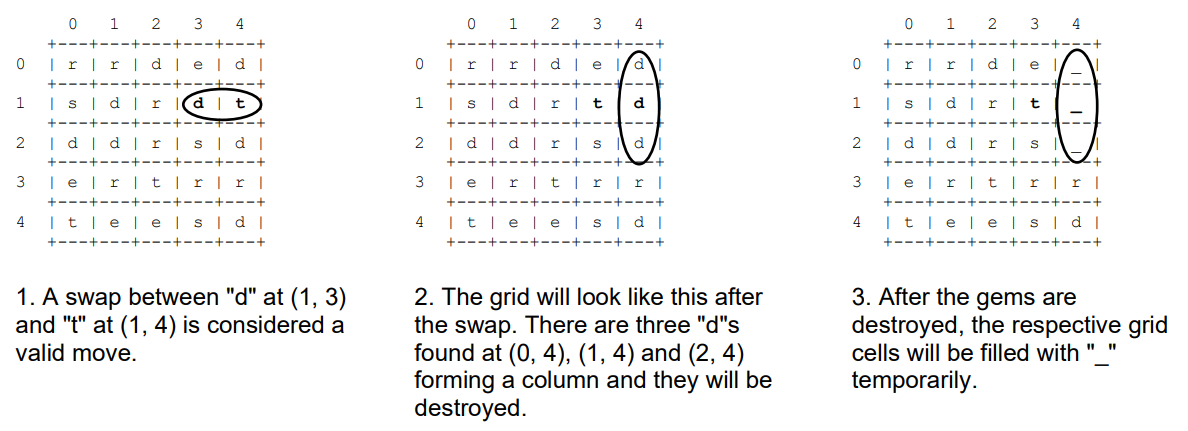
\includegraphics[width=0.7\paperwidth]{C:/Users/Admin/Desktop/Github/question_bank/LyX/static/img/9597-RVHS-2019-P1-Q4-1}
\par\end{center}

Some other valid swaps are: 
\begin{center}
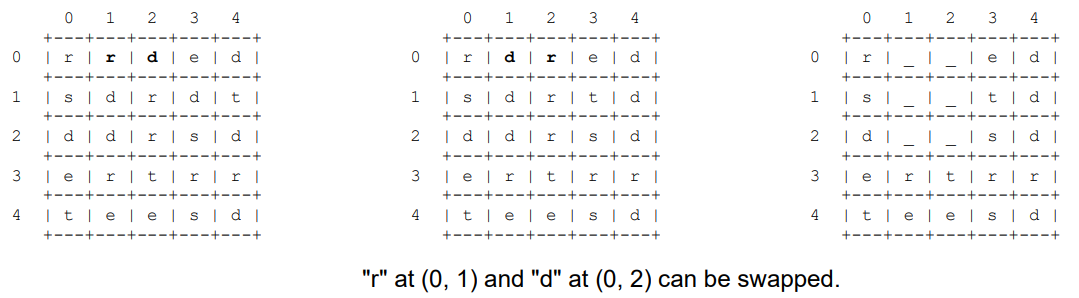
\includegraphics[width=0.7\paperwidth]{C:/Users/Admin/Desktop/Github/question_bank/LyX/static/img/9597-RVHS-2019-P1-Q4-2}
\par\end{center}

\begin{center}
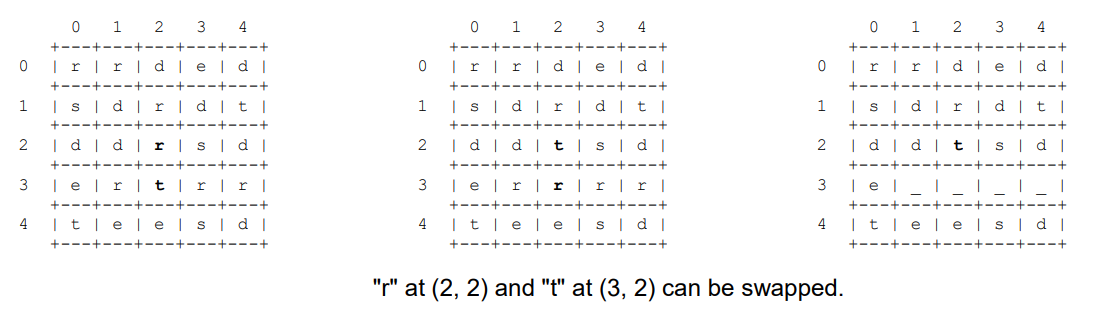
\includegraphics[width=0.7\paperwidth]{C:/Users/Admin/Desktop/Github/question_bank/LyX/static/img/9597-RVHS-2019-P1-Q4-3}
\par\end{center}

\begin{center}
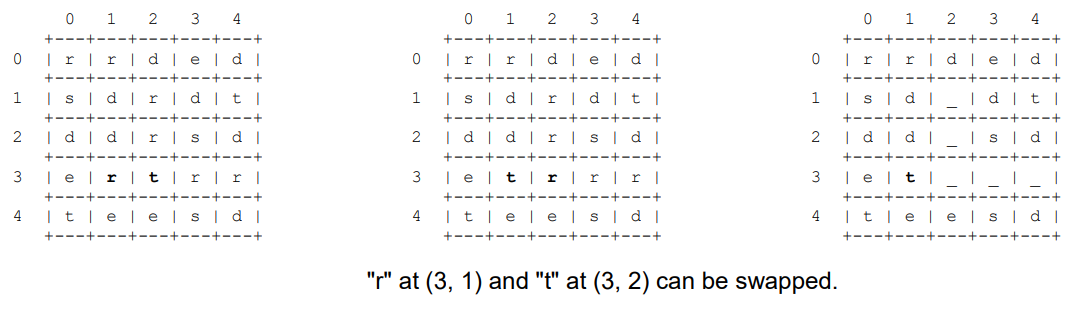
\includegraphics[width=0.7\paperwidth]{C:/Users/Admin/Desktop/Github/question_bank/LyX/static/img/9597-RVHS-2019-P1-Q4-4}
\par\end{center}

You are tasked to create a text-based interactive \textquotedblleft Begemed\textquotedblright{}
game in the following tasks. 

\subsection*{Task 4.1 }

Implement \texttt{Begemed} class according to the UML class diagram
and attributes/methods specifications given. 
\begin{center}
\begin{tabular}{|l|}
\hline 
\texttt{Board}\tabularnewline
\hline 
\texttt{- board: list }\tabularnewline
\hline 
\texttt{+ Board(size: int)}\tabularnewline
\texttt{+ new\_game(board: list) }\tabularnewline
\texttt{+ check\_connection(row: int, col: int): boolean }\tabularnewline
\texttt{+ find\_valid\_moves(row: int, col: int): list}\tabularnewline
\texttt{+ display(hint: boolean=False)}\tabularnewline
\hline 
\end{tabular}
\par\end{center}

\begin{center}
\begin{tabular}{|l|l|}
\hline 
\texttt{\textbf{Attribute}} & \texttt{\textbf{Specification}}\tabularnewline
\hline 
\texttt{board: list} & \texttt{board} is a 2-dimensional \texttt{list} hosting the gems inside
each grid. \tabularnewline
\hline 
\end{tabular}
\par\end{center}

Methods and its specification.
\begin{itemize}
\item \texttt{Board(n: int) : n} is the size used to define the dimension
of the \texttt{board}. The board should be initialized to a ($n\times n$)
2- dimensional list filled with string \textquotedblleft \_\textquotedblright .
\hfill{}{[}2{]}
\item \texttt{new\_game(new\_board : list): new\_game} takes in a \texttt{list}
named \texttt{new\_board} and assign it to the class attribute \texttt{board}.
The following list is provided in the python template file. 

t\texttt{est\_board = {[} {[}'r', 'r', 'd', 'e', 'd'{]}, {[}'s', 'd',
'r', 'd', 't'{]}, {[}'d', 'd', 'r', 's', 'd'{]}, {[}'e', 'r', 't',
'r', 'r'{]}, {[}'t', 'e', 'e', 's', 'd'{]}{]} }

\emph{This method is just a temporary solution which help you in initial
coding and debugging. In a later task, there will be further instructions
to update its implementation.} \hfill{}{[}1{]}
\item \texttt{check\_connection( row: int, col: int): boolean : check\_connection}
takes in the \texttt{row} and \texttt{col} value of a particular gem,
then check if there is a connection of 3 or more gems of the same
type in its horizontal or vertical direction. Return \texttt{True}
if such a connection is found, and \texttt{False} otherwise. \hfill{}{[}8{]}
\end{itemize}

\subsection*{Evidence 24 }

Program code of class Board and class methods up to \texttt{check\_conection}.
{[}11{]} 

Methods and its specification.
\begin{itemize}
\item \texttt{find\_valid\_moves( row: int, col: int): list} : \texttt{find\_valid\_moves}
takes in the \texttt{row} and \texttt{col} value of a particular gem,
then attempt to swap in the four directions (up, down, left, right).
If there is a new connection of 3 or more gems of the same type formed,
record as a valid movement. 

Return a \texttt{list} containing all valid movements. An empty \texttt{list}
is to be returned if no valid movement is found. 

For example:

\noindent %
\noindent\begin{minipage}[t]{1\columnwidth}%
\texttt{~~~~0~~~1~~~2~~~3~~~4 }

\texttt{~~+-{}-{}-+-{}-{}-+-{}-{}-+-{}-{}-+-{}-{}-+ }

\texttt{0 | r | r | d | e | d | }

\texttt{~~+-{}-{}-+-{}-{}-+-{}-{}-+-{}-{}-+-{}-{}-+ }

\texttt{1 | s | d | r | d | t | }

\texttt{~~+-{}-{}-+-{}-{}-+-{}-{}-+-{}-{}-+-{}-{}-+ }

\texttt{2 | d | d | r | s | d | }

\texttt{~~+-{}-{}-+-{}-{}-+-{}-{}-+-{}-{}-+-{}-{}-+ }

\texttt{3 | e | r | t | r | r | }

\texttt{~~+-{}-{}-+-{}-{}-+-{}-{}-+-{}-{}-+-{}-{}-+ }

\texttt{4 | t | e | e | s | d | }

\texttt{~~+-{}-{}-+-{}-{}-+-{}-{}-+-{}-{}-+-{}-{}-+ }%
\end{minipage}

If \texttt{find\_valid\_moves(0, 2)} is called, the function should
return \texttt{{[}'d', 'l'{]}} because when down swap or left swap
is performed on gem at \texttt{(0, 2)}, a new connection of 3 or more
gems of the same type will be formed. {[}5{]}
\item \texttt{display(hint: Boolean=False)} : \texttt{display} will print
out the \texttt{board} according to the sample format given. Take
note that the \texttt{size} of the board can be changed and hence
the grid outline should be dynamically adjusted according to its \texttt{size}. 

For example: 

\noindent %
\noindent\begin{minipage}[t]{1\columnwidth}%
\texttt{~~~~0~~~1~~~2~~~3~~~4}

\texttt{~~+-{}-{}-+-{}-{}-+-{}-{}-+-{}-{}-+-{}-{}-+}

\texttt{0 | r | r | d | e | d |}

\texttt{~~+-{}-{}-+-{}-{}-+-{}-{}-+-{}-{}-+-{}-{}-+}

\texttt{1 | s | d | r | d | t |}

\texttt{~~+-{}-{}-+-{}-{}-+-{}-{}-+-{}-{}-+-{}-{}-+}

\texttt{2 | d | d | r | s | d |}

\texttt{~~+-{}-{}-+-{}-{}-+-{}-{}-+-{}-{}-+-{}-{}-+}

\texttt{3 | e | r | t | r | r |}

\texttt{~~+-{}-{}-+-{}-{}-+-{}-{}-+-{}-{}-+-{}-{}-+}

\texttt{4 | t | e | e | s | d |}

\texttt{~~+-{}-{}-+-{}-{}-+-{}-{}-+-{}-{}-+-{}-{}-+}%
\end{minipage}

\texttt{hint} is an optional argument with a default value of \texttt{False}.
If \texttt{hint} is set to be \texttt{True}, the gems with valid moves
should be highlighted by using the \textbf{uppercase} letters, and
the valid moves for the \textbf{coordinates} and \textbf{directions}
should be displayed too. 

For example: 

\noindent %
\noindent\begin{minipage}[t]{1\columnwidth}%
\texttt{(0, 1) {[}'r'{]}}

\texttt{(0, 2) {[}'d', 'l'{]}}

\texttt{(1, 2) {[}'u'{]} }

\texttt{(1, 3) {[}'u', 'r'{]}}

\texttt{(2, 2) {[}'d'{]} }

\texttt{(3, 0) {[}'d'{]} }

\texttt{(3, 1) {[}'r'{]}}

\texttt{(3, 3) {[}'l'{]} }%
\end{minipage}

\noindent %
\noindent\begin{minipage}[t]{1\columnwidth}%
\texttt{~~~~0~~~1~~~2~~~3~~~4}

\texttt{~~+-{}-{}-+-{}-{}-+-{}-{}-+-{}-{}-+-{}-{}-+}

\texttt{0 | r | }\texttt{\textbf{\uline{R}}}\texttt{ | }\texttt{\textbf{\uline{D}}}\texttt{
| e | d |}

\texttt{~~+-{}-{}-+-{}-{}-+-{}-{}-+-{}-{}-+-{}-{}-+}

\texttt{1 | s | d | }\texttt{\textbf{\uline{R}}}\texttt{ | }\texttt{\textbf{\uline{D}}}\texttt{
| t |}

\texttt{~~+-{}-{}-+-{}-{}-+-{}-{}-+-{}-{}-+-{}-{}-+}

\texttt{2 | d | d | }\texttt{\textbf{\uline{R}}}\texttt{ | s |
d |}

\texttt{~~+-{}-{}-+-{}-{}-+-{}-{}-+-{}-{}-+-{}-{}-+}

\texttt{3 | }\texttt{\textbf{\uline{E}}}\texttt{ | }\texttt{\textbf{\uline{R}}}\texttt{
| t | }\texttt{\textbf{\uline{R}}}\texttt{ | r |}

\texttt{~~+-{}-{}-+-{}-{}-+-{}-{}-+-{}-{}-+-{}-{}-+}

\texttt{4 | t | e | e | s | d |}

\texttt{~~+-{}-{}-+-{}-{}-+-{}-{}-+-{}-{}-+-{}-{}-+}%
\end{minipage}
\end{itemize}

\subsection*{Evidence 25 }

Program code of class method \texttt{find\_valid\_moves} and \texttt{display}.
\hfill{}{[}14{]}

\subsection*{Task 4.2 }

Write a texted based menu which has the following options. Validation
of the user input is needed. 

\noindent %
\noindent\begin{minipage}[t]{1\columnwidth}%
\texttt{Choose an option below: }

\texttt{1) Validate Move }

\texttt{2) Toggle Hint Mode}

\texttt{3) Move the Gem!}

\texttt{4) New Game}

\texttt{5) Exit }%
\end{minipage}

The descriptions for the options can be found below. 

Options and its descriptions.
\begin{itemize}
\item \texttt{Validate Move} : Ask user to input a set of \texttt{row},
\texttt{col} and \texttt{direction}. Check and feedback if this swap
is valid. 
\item \texttt{Toggle Hint Mode} : For every new game, the \texttt{hint}
mode by default should be \texttt{off}. Use this option to toggle
the \texttt{on} and \texttt{off} state of hint mode.

If \texttt{hint} mode is \texttt{on}, the menu interface should automatically
highlight the gems with valid moves and print out a list of the coordinates
together with its valid movement directions. 
\item \texttt{Move the Gem! :} Move a gem in a chosen direction. 

\emph{Note that the related class method will only be implemented
in the }\textbf{\emph{next task}}\emph{. For the current menu, you
only need to take in user input for }\texttt{row}\emph{, }\texttt{col}\emph{
and }\texttt{direction}\emph{, but no further action needs to be taken. }
\item \texttt{New Game} : Start a new game and reset \texttt{hint} mode
to be off. 

For this task, you may just initialize the new game using the \texttt{test\_board}
given. 
\item \texttt{Exit} : Exit program. 
\end{itemize}

\subsection*{Evidence 26}

Program code of menu implementation. \hfill{}{[}10{]}

\subsection*{Task 4.3}

Update the class Begemed with the following methods. Note that this
task is time consuming and only worth \textbf{2 marks}. 

Methods and its specification.
\begin{itemize}
\item \texttt{new\_game(n: int)} : \texttt{new\_game} will now take in a
size of \texttt{n} and randomly generate a \texttt{$\mathtt{n}\times\mathtt{n}$}
board of gems. The newly generated gems should not have any connection
of 3 or more gems with the same type. 
\item \texttt{move\_gem(row: int, col: int, direction: string)} \texttt{move\_gem}
should take in a gem position and direction. If the swap is a valid
move, detect any newly formed connection of 3 or more gems with the
same type and cancel them. 

\noindent %
\begin{minipage}[t]{0.5\columnwidth}%
\texttt{~~~~0~~~1~~~2~~~3~~~4 }

\texttt{~~+-{}-{}-+-{}-{}-+-{}-{}-+-{}-{}-+-{}-{}-+ }

\texttt{0 | r | r | d | e | d |}

\texttt{~~+-{}-{}-+-{}-{}-+-{}-{}-+-{}-{}-+-{}-{}-+ }

\texttt{1 | s | d | r | d | t |}

\texttt{~~+-{}-{}-+-{}-{}-+-{}-{}-+-{}-{}-+-{}-{}-+ }

\texttt{2 | d | d | r | s | d |}

\texttt{~~+-{}-{}-+-{}-{}-+-{}-{}-+-{}-{}-+-{}-{}-+ }

\texttt{3 | e | }\texttt{\textbf{\uline{r}}}\texttt{ | }\texttt{\textbf{\uline{t}}}\texttt{
| r | r |}

\texttt{~~+-{}-{}-+-{}-{}-+-{}-{}-+-{}-{}-+-{}-{}-+ }

\texttt{4 | t | e | e | s | d |}

\texttt{~~+-{}-{}-+-{}-{}-+-{}-{}-+-{}-{}-+-{}-{}-+}

Swap \textquotedbl r\textquotedbl{} at (3, 1) with \textquotedbl t\textquotedbl{}
at (3, 2)%
\end{minipage}%
\begin{minipage}[t]{0.5\columnwidth}%
\texttt{~~~~0~~~1~~~2~~~3~~~4 }

\texttt{~~+-{}-{}-+-{}-{}-+-{}-{}-+-{}-{}-+-{}-{}-+}

\texttt{0 | r | r | d | e | d | }

\texttt{~~+-{}-{}-+-{}-{}-+-{}-{}-+-{}-{}-+-{}-{}-+ }

\texttt{1 | s | d | \_ | d | t |}

\texttt{~~+-{}-{}-+-{}-{}-+-{}-{}-+-{}-{}-+-{}-{}-+ }

\texttt{2 | d | d | \_ | s | d | }

\texttt{~~+-{}-{}-+-{}-{}-+-{}-{}-+-{}-{}-+-{}-{}-+ }

\texttt{3 | e | t | \_ | \_ | \_ | }

\texttt{~~+-{}-{}-+-{}-{}-+-{}-{}-+-{}-{}-+-{}-{}-+ }

\texttt{4 | t | e | e | s | d | }

\texttt{~~+-{}-{}-+-{}-{}-+-{}-{}-+-{}-{}-+-{}-{}-+}

Gems connected with 3 or more of the same type are cancelled. %
\end{minipage}

After the gems are being cancelled, those gems on top of the current
gems should \textquotedblleft fall\textquotedblright{} down. 

New gems will be randomly generated to fill up the board. 

\noindent %
\begin{minipage}[t]{0.5\columnwidth}%
\texttt{~~~~0~~~1~~~2~~~3~~~4 }

\texttt{~~+-{}-{}-+-{}-{}-+-{}-{}-+-{}-{}-+-{}-{}-+ }

\texttt{0 | r | r | \_ | \_ | \_ | }

\texttt{~~+-{}-{}-+-{}-{}-+-{}-{}-+-{}-{}-+-{}-{}-+ }

\texttt{1 | s | d | \_ | }\texttt{\textbf{\uline{e}}}\texttt{ |
}\texttt{\textbf{\uline{d}}}\texttt{ |}

\texttt{~~+-{}-{}-+-{}-{}-+-{}-{}-+-{}-{}-+-{}-{}-+ }

\texttt{2 | d | d | \_ | }\texttt{\textbf{\uline{d}}}\texttt{ |
}\texttt{\textbf{\uline{t}}}\texttt{ |}

\texttt{~~+-{}-{}-+-{}-{}-+-{}-{}-+-{}-{}-+-{}-{}-+ }

\texttt{3 | e | t | }\texttt{\textbf{\uline{d}}}\texttt{ | }\texttt{\textbf{\uline{s}}}\texttt{
| }\texttt{\textbf{\uline{d}}}\texttt{ |}

\texttt{~~+-{}-{}-+-{}-{}-+-{}-{}-+-{}-{}-+-{}-{}-+ }

\texttt{4 | t | e | e | s | d | }

\texttt{~~+-{}-{}-+-{}-{}-+-{}-{}-+-{}-{}-+-{}-{}-+ }

Gems on top of the cancelled gem \textquotedblleft falls\textquotedblright{}
down%
\end{minipage}%
\begin{minipage}[t]{0.5\columnwidth}%
\texttt{~~~~0~~~1~~~2~~~3~~~4 }

\texttt{~~+-{}-{}-+-{}-{}-+-{}-{}-+-{}-{}-+-{}-{}-+ }

\texttt{0 | r | r | }\texttt{\textbf{\uline{r}}}\texttt{ | }\texttt{\textbf{\uline{s}}}\texttt{
| }\texttt{\textbf{\uline{s}}}\texttt{ |}

\texttt{~~+-{}-{}-+-{}-{}-+-{}-{}-+-{}-{}-+-{}-{}-+ }

\texttt{1 | s | d | }\texttt{\textbf{\uline{t}}}\texttt{ | e |
d | }

\texttt{~~+-{}-{}-+-{}-{}-+-{}-{}-+-{}-{}-+-{}-{}-+ }

\texttt{2 | d | d | }\texttt{\textbf{\uline{t}}}\texttt{ | d |
t | }

\texttt{~~+-{}-{}-+-{}-{}-+-{}-{}-+-{}-{}-+-{}-{}-+ }

\texttt{3 | e | t | d | s | d |}

\texttt{~~+-{}-{}-+-{}-{}-+-{}-{}-+-{}-{}-+-{}-{}-+ }

\texttt{4 | t | e | e | s | d |}

\texttt{~~+-{}-{}-+-{}-{}-+-{}-{}-+-{}-{}-+-{}-{}-+ }

New gems are generated %
\end{minipage}

Check if there are more connections of 3 or more gems of the same
type are formed, if found repeat the above cancel and refill steps. 
\item \texttt{menu} Adjust the menu to accommodate these new changes. 
\end{itemize}

\subsection*{Evidence 27 }

Program code of above mentioned changes. \hfill{}{[}2{]}

{[}SPLIT\_HERE{]}
\item \textbf{{[}RVHS/PRELIM/9597/2019/P2/Q1{]} }

Vending machine
\begin{enumerate}
\item Draw a data flow diagram for a vending machine system that allows
user to buy drinks using coins and seller to refill stock. \emph{Note:
You are to decide on the processes to be included in the DFD on your
own}. \hfill{}{[}5{]}
\item Draw a flow chart on the steps in dispensing a drink by the vending
machine. Your flow chart should include various situations faced by
the system e.g. not enough cash, drinks chosen out of stock etc. \hfill{}{[}5{]}
\end{enumerate}
{[}SPLIT\_HERE{]}
\item \textbf{{[}RVHS/PRELIM/9597/2019/P2/Q2{]} }

Driverless car
\begin{enumerate}
\item State one ethical and one social issue of using driverless car. \hfill{}{[}2{]}
\item A simplified decision making on the behavior of a driverless car is
as follow. 
\begin{itemize}
\item When a pedestrian is sensed 10m ahead, the driverless car \textbf{must}
apply emergency break if its current speed is more than 20 km/hr.
Otherwise, it should slow down gently.
\item In other situations, when red light is sensed 20m ahead, the driverless
car should slow down gently regardless of its speed. 
\end{itemize}
Draw a reduced decision table for the scenario above. \hfill{}{[}5{]}
\end{enumerate}
{[}SPLIT\_HERE{]}
\item \textbf{{[}RVHS/PRELIM/9597/2019/P2/Q3{]} }

A project manager uses the PERT chart to manage a software project.
\begin{center}
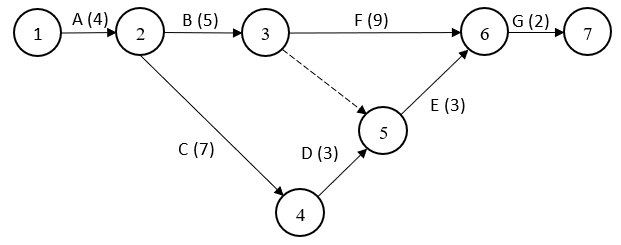
\includegraphics[width=0.5\paperwidth]{C:/Users/Admin/Desktop/Github/question_bank/LyX/static/img/9597-RVHS-2019-P2-Q3-1}
\par\end{center}

\noindent \begin{center}
\begin{tabular}{|c|c|c|}
\hline 
\textbf{Activity} & \textbf{Description} & \textbf{Duration (week)}\tabularnewline
\hline 
A & Specification & 4\tabularnewline
\hline 
B & Installation of datastore servers & 5\tabularnewline
\hline 
C & Development & 7\tabularnewline
\hline 
D & Unit Testing & 3\tabularnewline
\hline 
E & System testing & 3\tabularnewline
\hline 
F & Conversion of existing data files to new format & 9\tabularnewline
\hline 
G & UAT & 2\tabularnewline
\hline 
\end{tabular}
\par\end{center}
\begin{enumerate}
\item Explain the significance of the dotted line. \hfill{}{[}1{]}
\item Draw a Gantt chart based on the above information.\hfill{} {[}3{]}
\item State the impact on the project if activity F duration is cut by 3
weeks.\hfill{} {[}2{]}
\item State the purpose of the project proposal.\hfill{} {[}1{]}
\item State 2 important topics in the project proposal. \hfill{}{[}1{]}
\end{enumerate}
{[}SPLIT\_HERE{]}
\item \textbf{{[}RVHS/PRELIM/9597/2019/P2/Q4{]} }

A user-defined linked list has the following operations.

Operations and its descriptions 
\begin{itemize}
\item \texttt{create()} : This function creates an empty linked list.

For example: 

\texttt{lst1 = create()}

A linked list is created and referenced by \texttt{lst1}.
\item \texttt{insert(llst,data)} : This procedure always adds \texttt{data}
as a node at the head of the linked list

For example

\noindent %
\noindent\begin{minipage}[t]{1\columnwidth}%
\texttt{lst1: 'A'->'B'->'C'->'D'->'E'}

\texttt{insert(lst1, 'Z')}

\texttt{lst1: 'Z'->'A'->'B'->'C'->'D'->'E'}%
\end{minipage}
\item \texttt{split(llst,pos)} The function breaks the linked list at position
\texttt{pos} and returns the cut half as a new linked list.

For example: 

\noindent %
\noindent\begin{minipage}[t]{1\columnwidth}%
\texttt{lst1: 'A'->'B'->'C'->'D'->'E'}

\texttt{lst2 = split(lst1, 2)}

\texttt{lst1: 'A'->'B' }

\texttt{lst2: 'C'->'D'->'E'}%
\end{minipage}
\item \texttt{join(llst1,llist2)} This function joins 2 linked lists as
one.

For example: 

\noindent %
\noindent\begin{minipage}[t]{1\columnwidth}%
\texttt{lst1: 'C'->'B' }

\texttt{lst2: 'A'->'D'->'E}

\texttt{join(lst1, lst2)}

\texttt{lst1: 'C'->'B'->'A'->'D'->'E' }

\texttt{lst2: Empty}%
\end{minipage}
\end{itemize}
Using the provided operations of the linked list, write, in pseudo-code
an algorithm that could be used to implement the \texttt{swap} operation.
\emph{Hint: you don\textquoteright t have to use all the operations
provided}.

Operations and its description 
\begin{itemize}
\item \texttt{swap(llst,pos)} : This procedure swaps the data at positions
\texttt{pos} and \texttt{pos + 1}

For example: 

\noindent %
\noindent\begin{minipage}[t]{1\columnwidth}%
\texttt{lst1:'A'->'B'->'C'->'D'->'E' }

\texttt{swap(lst1,3)}

\texttt{lst1:'A'->'B'->'D'->'C'->'E'}%
\end{minipage}
\end{itemize}
You can assume that the operations executed are always valid. For
example, if there is no 5th node, \texttt{swap(lst1,4)} will not be
called. \hfill{}{[}5{]}

{[}SPLIT\_HERE{]}
\item \textbf{{[}RVHS/PRELIM/9597/2019/P2/Q5{]} }

Computer Network
\begin{enumerate}
\item Explain how the switch forwards data packet to destinated device.
\hfill{}{[}1{]}
\item State the function of a router.\hfill{} {[}1{]}
\item Explain with an example what a client server network is.\hfill{}
{[}1{]}
\item Describe the differences between PaaS and IaaS.\hfill{} {[}1{]}
\item State 2 data verification methods.\hfill{} {[}1{]}
\item Explain what packet switching is.\hfill{} {[}1{]}
\item State the connection mode that the walkie-talkie (push to talk) is
working on.\hfill{} {[}1{]}
\item State the difference between synchronous and asynchronous data transmission.
\hfill{}{[}1{]}
\item State and explain a method to protect data in transit.\hfill{} {[}1{]}
\item State and explain a method to protect data at rest.\hfill{}{[}1{]}
\end{enumerate}
{[}SPLIT\_HERE{]}
\item \textbf{{[}RVHS/PRELIM/9597/2019/P2/Q6{]} }

A sort procedure is implemented in Python is follow.

\noindent %
\noindent\begin{minipage}[t]{1\columnwidth}%
\texttt{def sort(sort\_lst, unsort\_lst):}

\texttt{\qquad{}if len(unsort\_lst) > 0: }

\texttt{\qquad{}\qquad{}item = unsort\_lst{[}0{]} }

\texttt{\qquad{}\qquad{}i = 0 }

\texttt{\qquad{}\qquad{}while i < len(sort\_lst) and item < sort\_lst{[}i{]}: }

\texttt{\qquad{}\qquad{}\qquad{}i += 1 }

\texttt{\qquad{}\qquad{}return sort(sort\_lst{[}:i{]}+{[}item,{]}+sort\_lst{[}i:{]},
unsort\_lst{[}1:{]})}

\texttt{\qquad{}else:}

\texttt{\qquad{}\qquad{}return sort\_lst}%
\end{minipage}
\begin{enumerate}
\item State the name of the above sorting algorithm. \hfill{}{[}1{]}
\item The below statement is executed.

\texttt{>\textcompwordmark >\textcompwordmark > sort({[}{]}, {[}9,1,8,2,3,7,5{]})}

Using the table below, trace the items in \texttt{sort\_lst} and \texttt{unsort\_lst}
in each recursive call.
\noindent \begin{center}
\begin{tabular}{|c|c|c|}
\hline 
\texttt{\textbf{\#}} & \texttt{\textbf{sort\_lst}} & \texttt{\textbf{unsort\_lst}}\tabularnewline
\hline 
\texttt{1} & \texttt{{[}{]}} & \texttt{{[}9,1,8,2,3,7,5{]}}\tabularnewline
\hline 
\texttt{2} &  & \tabularnewline
\hline 
\texttt{3} &  & \tabularnewline
\hline 
\texttt{4} &  & \tabularnewline
\hline 
\texttt{5} &  & \tabularnewline
\hline 
\texttt{6} &  & \tabularnewline
\hline 
\texttt{7} &  & \tabularnewline
\hline 
\texttt{8} &  & \tabularnewline
\hline 
\end{tabular}
\par\end{center}

\hfill{}{[}3{]}
\item State the time complexity of the sort procedure above. \hfill{}{[}1{]}
\end{enumerate}
\quad{} A sleepy teacher implemented an inefficient binary search
function as follow. The function is supposed to return True if target
is found in the list inc\_sort\_lst and False otherwise.

\noindent %
\noindent\begin{minipage}[t]{1\columnwidth}%
\texttt{01 def binSearch(target, inc\_sort\_lst):}

\texttt{02 if len(inc\_sort\_lst) == 0: }

\texttt{03 \qquad{}return False}

\texttt{04 if len(inc\_sort\_lst) == 1: }

\texttt{05 \qquad{}return True }

\texttt{06 n = len(inc\_sort\_lst)}

\texttt{07 first\_half = inc\_sort\_lst{[}:n//2{]} }

\texttt{08 second\_half = inc\_sort\_lst{[}n//2:{]} }

\texttt{09 if target > first\_half{[}-1{]}: }

\texttt{10 \qquad{}return binSearch(target, second\_half) }

\texttt{11 else: }

\texttt{12 \qquad{}return binSearch(target, first\_half)}%
\end{minipage}
\begin{enumerate}
\item[(d)]  Explain the bug in his code with examples. \hfill{}{[}1{]}
\item[(e)]  Explain how you can correct the bug without changing the code from
line 06 onwards.\hfill{} {[}2{]}
\item[(f)]  Explain why the binary search performed is inefficient.\hfill{}
{[}2{]}
\end{enumerate}
{[}SPLIT\_HERE{]}
\item \textbf{{[}RVHS/PRELIM/9597/2019/P2/Q7{]} }

Run length encoding (RLE) is a very simple form of lossless data compression
which runs on sequences having same value occurring many consecutive
times and it encodes the sequence to store only a single value and
its count. For example, \textquotedblleft 111111000\textquotedblright{}
can be converted to \textquotedblleft 6130\textquotedblright .

Below is a draft attempt of implementing this algorithm. 

\noindent %
\noindent\begin{minipage}[t]{1\columnwidth}%
\texttt{01 PROCEDURE RLECompress(s: STRING): }

\texttt{02 \qquad{}DECLARE comp\_str: STRING }

\texttt{03 \qquad{}DECLARE count, i: INT }

\texttt{04 \qquad{}comp\_str = \textquotedbl\textquotedbl{} }

\texttt{05 \qquad{}count, i = 0, 0 }

\texttt{06 }

\texttt{07 \qquad{}WHILE i < LENGTH(s): }

\texttt{08 \qquad{}\qquad{}count = 1 }

\texttt{09 }

\texttt{10 \qquad{}\qquad{}WHILE i < LENGTH(s) - 1 and s{[}i{]}
== s{[}i+1{]}:}

\texttt{11 \qquad{}\qquad{}\qquad{}count += 1 }

\texttt{12 \qquad{}\qquad{}\qquad{}i += 1 }

\texttt{13 \qquad{}\qquad{}END WHILE }

\texttt{14 }

\texttt{15 \qquad{}\qquad{}comp\_str += count + s{[}i{]} }

\texttt{16 \qquad{}END WHILE }

\texttt{17 }

\texttt{18 \qquad{}RETURN comp\_str }

\texttt{19 END PROCEDURE}%
\end{minipage}
\begin{enumerate}
\item The compiler reported an error at line 15. Identity the type of error,
state its definition and suggest how it can be fixed.\hfill{} {[}3{]}
\item After the above error has been corrected, a successful compilation
produces executable code. However, when the code was executed, it
failed to complete. Identity another type of error, state its definition
and suggest how it can be fixed. \hfill{}{[}3{]}
\end{enumerate}
Assuming all errors have been identified and corrected.

The following steps are taken to encode English alphabets:
\begin{enumerate}
\item[1.]  Convert alphabet to hexadecimal ASCII value 
\item[2.]  Convert the hexadecimal number to binary number 
\item[3.]  Encode the binary number using RLE algorithm
\end{enumerate}
For example, the alphabet \textquotedblleft A\textquotedblright{}
has a hexadecimal ASCII value of \textquotedblleft 41\textquotedblright .
\begin{enumerate}
\item[(c)]  State the definition of ASCII.\hfill{} {[}2{]}
\item[(d)]  State the encoded RLE string for letter \textquotedblleft A\textquotedblright .\hfill{}
{[}1{]}
\item[(e)]  State and explain with example one potential limitation of RLE encoding
when compressing long binary strings. \hfill{}{[}2{]}
\end{enumerate}
{[}SPLIT\_HERE{]}
\item \textbf{{[}RVHS/PRELIM/9597/2019/P2/Q8{]} }

The school library currently stores their data in flat files. These
files contain information about students, books and their loaning
details. 

Using examples from the school\textquoteright s flat files to illustrate
your answers.
\begin{enumerate}
\item Explain how data inconsistency could arise.\hfill{} {[}2{]}
\item Explain why data privacy could be a potential concern.\hfill{} {[}2{]}
\item Explain the definition of Primary Key in a relational database. \hfill{}{[}2{]}
\end{enumerate}
A book can be borrowed by any student, and a student can borrow any
book. Students need to fill up a loaning record form each time he/she
wants to borrow a book. A student is entitled to borrow up to 5 books
each time using the same loaning record form.

The decision has been made to create a relational database for the
library loaning system.
\begin{enumerate}
\item[(d)]  Identify the necessary tables and draw an E-R diagram to show the
relationships between these tables. {[}4{]}
\item[(e)]  For each table specify the attributes (fields) required and state
suitable primary keys and foreign key relationships. State necessary
legends if you are using symbols to represent the primary and foreign
keys. {[}7{]}
\end{enumerate}
The following table is generated for students\textquoteright{} reference
regarding their loaning details.

\begin{tabular}{|l|l|l|l|}
\hline 
\textbf{Student Name:} & Xiao Ming  & \textbf{Class: } & 19J08\tabularnewline
\hline 
 &  &  & \tabularnewline
\hline 
\textbf{Book Name} & \textbf{Author} & \textbf{Loan Date} & \textbf{Due Date}\tabularnewline
\hline 
A Brief History of Time & Stephen Hawking & 05 Aug 2019 & 30 Aug 2019\tabularnewline
\hline 
Spider Man Comics & Stan Lee & 29 Aug 2019 & 20 Sep 2019\tabularnewline
\hline 
\end{tabular}
\begin{enumerate}
\item[(f)]  To create the report \texttt{StudentName} and \texttt{StudentClass}
are used. Name other fields that the database uses to produce this
report.\hfill{}{[}4{]}
\end{enumerate}
Beside the database design, you are also in charge of creating an
online loaning form.
\begin{enumerate}
\item[(g)]  Design and draw a webpage layout for the auto loaning interface
for the new system. Identify and briefly explain your design considerations
for the various features which aid users to input valid data entries.
\hfill{}{[}4{]}
\item[(h)]  Some students use their handphones to snap photos of tables and
charts from the books they borrowed and use them for their research
projects. Explain what potential issues may arise and suggest alternate
ways which students can adopt.\hfill{} {[}3{]}
\end{enumerate}
{[}SPLIT\_HERE{]}
\item \textbf{{[}RVHS/PRELIM/9597/2019/P2/Q9{]} }

The school library has in store different kinds of items which students
can loan out. Information about items are stored and recorded, such
as \texttt{title}, \texttt{description}, and \texttt{damaged}, which
is a Boolean value indicating if the item has any form of physical
damage.

For books in the library, additional information such as the \texttt{author},
\texttt{publisher}, \texttt{ISBN} are recorded.

Digital media resources are also available for students\textquoteright{}
reference. Information such as \texttt{storage media}, \texttt{file
size} and\texttt{ playback time} are stored. 

You are engaged by the school to design an Object-Oriented Programming
solution to manage these items.
\begin{enumerate}
\item Draw a class diagram, with base class \texttt{Item}, showing: 
\begin{itemize}
\item appropriate sub-classes 
\item inheritance
\item the properties required 
\item appropriate methods, including \textbf{constructor} methods, and at
least \textbf{one} pair of \textquoteleft \textbf{get}\textquoteright{}
and \textquoteleft \textbf{set}\textquoteright{} methods for one of
the properties. \hfill{}{[}5{]}
\end{itemize}
\item Using the above example, explain the meaning of the term \textbf{Polymorphism}.
\hfill{}{[}2{]}
\item Using the above example, explain the meaning of the term \textbf{Encapsulation}.\hfill{}
{[}2{]}
\item The school also provides a series of past year examination papers
for the students\textquoteright{} loaning and reference. State how
this would affect the \textbf{class}, \textbf{properties} and \textbf{methods}
in the current example. \hfill{}{[}2{]}
\end{enumerate}
{[}SPLIT\_HERE{]}
\end{enumerate}
 
\end{document}
